\chapter{Simulation Environments, Plugins, and Input Data}
\label{sec:simulation_environments_and_data}



LODUS is designed to model simulation scenarios using real-world spatial and demographic data. 
To evaluate this capability in an urban setting, we model the city of Porto Alegre and its population using three main representations. 
The first represents both population and points of interest ($P$s) at the neighborhood level. The second preserves neighborhoods as simulation regions while representing population and $P$s at the finer census-sector level across the entire city. The third uses the same census-sector-level representation but is restricted to 13 neighborhoods in the central area of Porto Alegre. 

In addition to environment and population data, service, flood, shelter, and behavioral datasets are overlaid on the representation appropriate to each use case. This chapter presents these environments and their shared inputs, distinguishing between observed or externally sourced data, data derived through spatial or statistical preprocessing, and values configured specifically for each simulation scenario.

%SO: re-escrevi. validar
%GA: validado
Following the model introduced in Chapter~\ref{chapter:proposed_model}, each input described in this chapter contributes either to the initialization of the core model or to the configuration of domain-specific plugins.
Core inputs define the simulation environment, the initial population, and the routines executed during the simulation. 
Plugin-specific inputs instead configure the parameters of a plugin, extend the core model with application-specific information, or provide the data required by the additional routines, actions, or simulation behaviors introduced by that plugin. 
This distinction separates the origin of an input from its role in the simulation, making it possible to reuse the same core model across different application domains.

%Following the definitions introduced in Chapter~\ref{chapter:proposed_model}, each input described in this chapter has one of two roles. Core inputs initialize point-of-interest types and attributes, population blobs and their characteristics, or local and global routines. Experiment-specific inputs instead configure plugins through $\bm{\theta}_{\Pi}$, extend the model vocabulary through $E_{\Pi}$, or provide data used by routine contributions, action handlers, and lifecycle hooks. This distinction separates the provenance of an input from the mechanism through which it affects the simulation.



\section{Spatial Representations}
\label{sec:spatial_representations}

Following the environment definition introduced in Section~\ref{sec:environment}, neighborhoods are modeled as simulation regions ($R$), each containing a set of $P$s. The environments differ primarily in their spatial extent and in the resolution at which population and $P$s are represented.


\subsection{Neighborhood-Level Environment}
\label{sec:neighborhood_level_environments}

The neighborhood-level Porto Alegre model follows the environment described in the published manuscript~\cite{silva2026lodusPop}. Each of the city's 94 neighborhoods is represented as a simulation region. 
Neighborhood boundaries were obtained from digital cartographic data published by Porto Alegre City Hall\footnote{Porto Alegre City Hall digital maps, including the neighborhood boundary layer (``Bairros (LC 12.112/16)''): \url{https://prefeitura.poa.br/carta-de-servicos/mapas-digitais-da-smamus}.}, while OpenStreetMap was used to obtain coordinates for urban amenities represented as $P$s\footnote{OpenStreetMap: \url{https://www.openstreetmap.org/}.}. 
Each region contains one $P$ of each standard type $\tau_i$: \textit{home}, \textit{work}, \textit{school}, \textit{marketplace}, \textit{pharmacy}, and \textit{gas station}.
Selected regions also contain $P$s with specialized types, such as shopping malls and stadiums, when required by an experiment. Coordinates, external identifiers, and other location-specific values are stored in the attribute mapping $\bm{\alpha}_i$ of each $P_i$.


Population totals, citywide occupation proportions, and the citywide age distribution were obtained from the 2010 Census of the Brazilian Institute of Geography and Statistics (IBGE)\footnote{IBGE city profile for Porto Alegre: \url{https://cidades.ibge.gov.br/brasil/rs/porto-alegre/panorama}.}. Neighborhood-level population and age distributions were complemented with municipal information published by ObservaPOA and PROCEMPA\footnote{ObservaPOA: \url{http://www.observapoa.com.br/}. PROCEMPA's Porto Alegre em Análise portal: \url{https://portoalegreemanalise.procempa.com.br/}.}.


One initial population blob is placed at the home $P$ of each neighborhood. Age and occupation are represented as sampled characteristics in $\bm{Sc}$, since each blob stores a distribution over their categories. Experiment-specific traceable characteristics, such as infection status, vaccination status, mobility lifecycle, or patient state, are introduced by the corresponding plugin through its model extensions ($E_{\Pi}$), which also define their
default values.

Occupation is divided into \textit{students}, \textit{workers}, and \textit{others}. Because neighborhood-level occupation distributions were unavailable, the same citywide distribution was applied to every neighborhood: approximately 21.6\% students, 54.7\% workers, and 23.7\% others. Age is divided into four categories: \textit{child} (0--14 years), \textit{young} (15--24 years), \textit{adult} (25--59 years), and \textit{elder} (60+ years). Each neighborhood uses its corresponding age distribution, while the overall modeled population consists of approximately 18.7\% children, 15.7\% young people, 50.5\% adults, and 15.1\% elders. Overall, the neighborhood-level environment comprises 94 $R$s, 504 $P$s, and a total population of 1,409,351.

\subsection{Census-Sector-Level Environments}
\label{sec:census_sector_environments}

The more detailed environments use census sectors, also referred to as enumeration areas, as the spatial unit for population initialization. Neighborhoods remain the simulation regions, preserving compatibility with region-level routines and outputs, while census sectors provide a finer spatial representation of the population and associated $P$s. Official census-sector aggregates and geographic files were obtained from the 2022 IBGE Census\footnote{IBGE 2022 Census sectors: \url{https://www.ibge.gov.br/geociencias/organizacao-do-territorio/malhas-territoriais/26565-malhas-de-setores-censitarios-divisoes-intramunicipais.html}.}.

The neighborhood-level environment described in the previous section was originally constructed using demographic data from the 2010 IBGE Census, consistent with the environment used in the published experiments~\cite{silva2026lodusPop}. The census-sector environments were subsequently constructed using the more recent 2022 Census data. %Consequently, differences in population totals between these environments reflect both their spatial representation and the underlying census datasets.


In both census-sector environments, six standard $P$s are instantiated for each census sector within the neighborhood region containing that sector. Their types ($\tau_i$) correspond to \textit{home}, \textit{work}, \textit{school}, \textit{marketplace}, \textit{pharmacy}, and \textit{restaurant}. The census sector is therefore the unit used to position and initialize these $P$s, whereas neighborhoods remain the simulation regions ($R$s). The population associated with each sector is initially represented by a blob at its corresponding \textit{home} $P$.

We consider two versions of this representation: a \textit{complete environment}, covering all 94 neighborhoods of Porto Alegre, and a \textit{reduced environment}, restricted to 13 neighborhoods in the central area of the city.
The complete environment applies this representation to 2,711 census sectors distributed across all 94 neighborhoods, resulting in 16,266 $P$s and a total population of 1,331,414. The reduced environment applies the same representation to 435 census sectors distributed across 13 central neighborhoods, resulting in 2,610 $P$s and a total population of 159,886.


Table~\ref{tbl:shared_simulation_environments} summarizes the three environment versions. The reported counts of $P$s refer to the base spatial representations. Domain-specific plugins may extend these environments with additional $P$s required by a scenario, such as shelters, dialysis clinics, and water-treatment facilities.
Figure~\ref{fig:spatial_representations} presents their spatial representations, highlighting the distribution of home $P$s. 
The main use cases are presented in the results chapter (Chapter~\ref{chapter:experimental_results}).

\begin{table}[ht]
\centering
\footnotesize
\setlength{\tabcolsep}{4pt}
\caption{Base Porto Alegre spatial representations used by the experiments.}
\label{tbl:shared_simulation_environments}
\begin{tabularx}{\linewidth}{@{}p{2.6cm}rrrrX@{}}
\toprule
\textbf{Environment} &
\textbf{Regions} &
\textbf{Home $P$s} &
\textbf{Base $P$s} &
\textbf{Population} &
\textbf{Main use cases} \\
\midrule
Neighborhood-level
    & 94 & 94 & 504 & 1,409,351
    & Published L\'evy Walk, large-scale events, epidemic contagion, and vaccination. \\
Reduced census-sector
    & 13 & 435 & 2,610
    & 159,886
    & Popular Times, L\'evy Walk, dialysis, and flood-aware mobility. \\
Complete census-sector 
    & 94 & 2,711 & 16,266
    & 1,331,414
    & Popular Times, L\'evy Walk, dialysis, and flood-aware mobility. \\
\bottomrule
\end{tabularx}
\end{table}

\begin{figure}[ht]
 \centering
  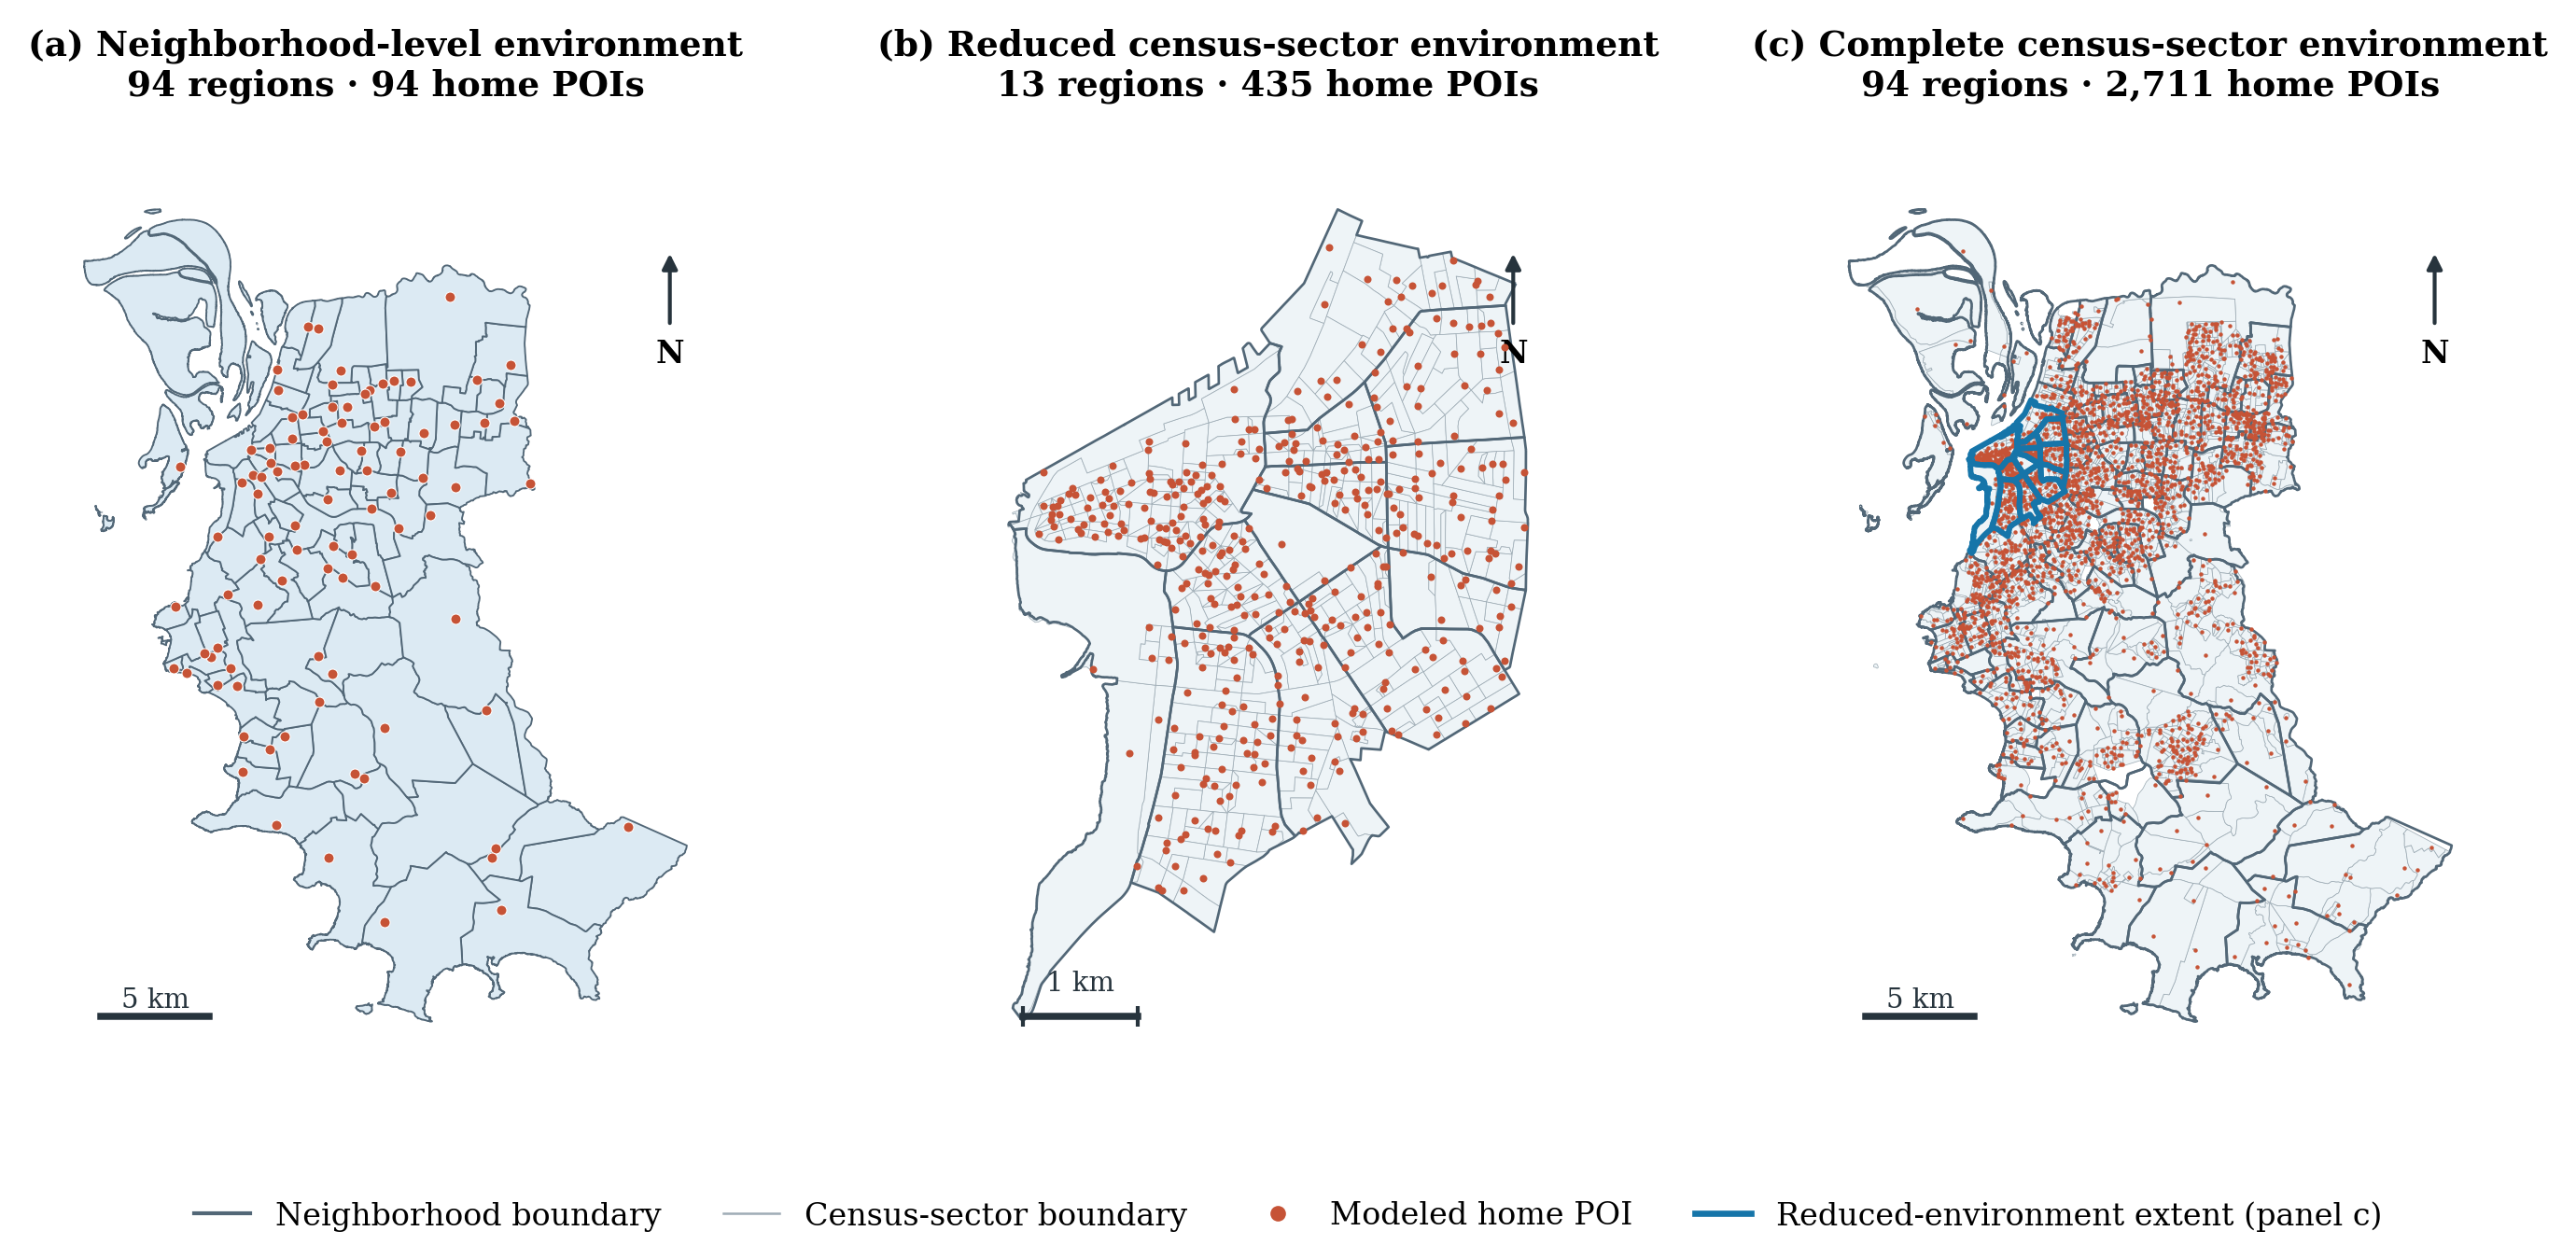
\includegraphics[width=0.99\textwidth]{fig/viz/spatial_environment_comparison.png}
  \caption{Spatial representations of Porto Alegre used in the experiments, highlighting the distribution of home $P$s in the neighborhood-level, reduced census-sector, and complete census-sector environments. The outlines in the complete environment represents the reduced environment’s 13-neighborhoods.}
  \label{fig:spatial_representations}
\end{figure}


\section{Implemented Plugins and Scenario-Specific Inputs}
\label{sec:scenario_specific_inputs}


The spatial representations introduced in the previous section provide the common environment and population basis for the experiments in this thesis. Different application scenarios, however, require additional data and simulation behavior beyond this shared representation. 
These requirements are introduced through domain-specific plugins, which extend the LODUS core model with the state, routines, actions, and simulation-step behavior needed to represent each phenomenon.

This section presents the implemented plugins together with the inputs used to configure and support them. The extensions address normal life mobility, large-scale events, environmental disruptions and shelters, contagion and vaccination, and dialysis services. 
For each case, we describe the role of the plugin, the principal contributions it introduces according to the model defined in Section~\ref{sec:extension_mechanism}, and the external, derived, or scenario-defined inputs required by its behavior. In addition to extending population state and simulation behavior, some plugins also augment the base spatial representations with domain-specific $P$s. 
In the extensions presented here, such additions include shelters, dialysis clinics, and water-treatment facilities. In this way, the section complements the shared environments described above by showing how they are extended and configured for the different experimental scenarios considered in this thesis.
%Table~\ref{tbl:input_plugin_mapping} connects these input families to the extension contract defined in Section~\ref{sec:plugins}. 
%Table~\ref{tbl:input_plugin_mapping} relates these input families to the plugin contributions introduced in Section~\ref{sec:plugins}. The mapping %SO: qual mapping?
%identifies the principal nonempty components used by each experiment family; individual experimental sections report the selected parameter values and policies in greater detail. Environment fields such as $\tau_i$, $\bm{\alpha}_i$, $C_i(t)$, and $D_i$ remain part of the core simulation state even when a plugin declares its conventions or modifies its values. 

\begin{comment}
    
%GA: toda ssa section foi reescrita
%SO: importante na tabela abaixo e em todo texto arrumar aquele "contract"
\begin{table}[ht]
\centering
\footnotesize
\setlength{\tabcolsep}{4pt}
\caption{Principal mapping %SO: correspondence???
from scenario-input families to the plugin extension contract.}
\label{tbl:input_plugin_mapping}
\begin{tabularx}{\linewidth}{@{}p{3.0cm}p{3.4cm}X@{}}
\toprule
\textbf{Experiment family} & \textbf{Principal components} & \textbf{Role of the inputs} \\
\midrule
Routine mobility
& $\bm{\theta}_{\Pi}$, $E_{\Pi}$, $\mathcal{F}_{\Pi}$, $\mathcal{H}_{\Pi}$
& Configures mobility distributions or temporal profiles, declares lifecycle characteristics, and supplies the handlers and step updates that generate and consume movement requests. \\
Large-scale events
& $\bm{\theta}_{\Pi}$, $\mathcal{R}_{\Pi}$, $\mathcal{F}_{\Pi}$
& Defines event times and demand volumes, schedules gathering requests, and consumes them through registered action handlers. \\
Contagion and vaccination
& $\bm{\theta}_{\Pi}$, $E_{\Pi}$, $\mathcal{F}_{\Pi}$, $\mathcal{H}_{\Pi}$
& Defines epidemiological and vaccination parameters, declares population states, and updates those states during execution. \\
Flooding and shelters
& $\bm{\theta}_{\Pi}$, $E_{\Pi}$, $\mathcal{F}_{\Pi}$, $\mathcal{H}_{\Pi}$
& Provides hazard and capacity parameters, declares $P$-attribute conventions and population states, and implements availability and displacement policies. \\
Dialysis services
& $\bm{\theta}_{\Pi}$, $E_{\Pi}$, $\mathcal{F}_{\Pi}$, $\mathcal{H}_{\Pi}$
& Configures recurring demand, clinic schedules and capacity, declares patient states, and implements treatment and return transitions. Clinic dependencies remain represented by $D_i$. \\
\bottomrule
\end{tabularx}
\end{table}
\end{comment}



\subsection{Normal-Life Mobility}
\label{sec:normal_life}

Normal life represents recurring population movements performed under ordinary conditions. These movements are introduced through two complementary mobility plugins: L\'evy Walk and Popular Times. The former generates mobility primarily from stochastic spatial displacement or attendance-based demand, while the latter generates mobility from temporally structured demand profiles associated with different categories of destinations. Together, they provide the baseline population movement upon which other processes, such as large-scale events, epidemic contagion, or environmental disruptions, may operate.

For clarity, the experiments distinguish between two forms of routine movement: \textit{commutes} and \textit{activities}. A \textit{commute} denotes a recurring trip associated with work or school, whereas an \textit{activity} denotes a visit to another urban location, such as a marketplace, restaurant, or pharmacy. These terms characterize the roles assigned to movements in the experiments rather than intrinsic restrictions of the corresponding plugins. 
In the configurations considered in this thesis, L\'evy Walk is primarily used to generate commutes, while Popular Times is used to generate activities. However, either plugin can be configured for other mobility purposes by changing the eligible population, destination types, temporal profiles, and related parameters.


\subsubsection{L\'evy Walk Plugin} 
\label{sec:levy_walk_plugin_inputs}

The \textit{L\'evy Walk Plugin} generates population movement using a stochastic spatial model in which travel distances follow a L\'evy distribution~\cite{levy_flight}. This produces many short-distance movements and progressively fewer long-distance movements, consistent with patterns reported for human mobility~\cite{gonzalez2008understanding}. The plugin does not prescribe a particular semantic purpose for these movements; eligible population groups and destination types are determined through its configuration. 
Rather than reproducing observed individual trajectories, the plugin generates mobility from configurable behavioral parameters, allowing controlled comparisons under different mobility conditions.

The plugin supports two forms of mobility generation. The configuration originally introduced with the published manuscript~\cite{silva2026lodusPop} divides eligible populations into configurable packets and evaluates their movement according to a movement probability. For each moving packet, a travel distance is sampled from the L\'evy distribution and used to select a destination within a corresponding distance interval. The principal inputs of this configuration therefore include the parameters of the L\'evy distribution, movement probability, population-packet size, destination types, and distance discretization. An optional mobility-restriction factor can additionally reduce the population selected for movement when required by a scenario.

For the census-sector environments, the plugin can instead generate demand according to explicit attendance rates. In this configuration, the eligible population expected to commute during a modeled day is determined from configurable attendance parameters and distributed among population origins and departure times according to temporal profiles. Additional configuration parameters determine population-packet limits, destination types, and the duration of each mobility episode.

Population templates determine which groups are eligible for each movement. In the commute configurations considered in this thesis, occupation and age characteristics are used to identify workers and students, while \textit{work} and \textit{school} $P$s provide their respective destinations. These associations are configuration choices and may be changed when the plugin is applied to other forms of mobility.

The attendance-based configuration additionally extends the population representation with traceable characteristics that preserve information about the movement lifecycle, including the original home, requested and receiving destinations, departure time, and scheduled return. These characteristics remain associated with population blobs as they are split, moved, and subsequently returned and merged, allowing requested, completed, and unmet movements to remain distinguishable during simulation execution.

%The specific L\'evy Walk parameters, temporal profiles, population groups, packet sizes, movement durations, and other configuration values adopted by each experiment are presented in the corresponding simulation setup.

\subsubsection{Popular Times Plugin}
\label{sec:popular_times_plugin_inputs}

The \textit{Popular Times Plugin} generates population movement according to temporal demand profiles associated with categories of $P$s. Rather than determining demand primarily from stochastic travel distances, the plugin represents how demand for a destination type varies according to the day of the week and hour of the day. As with L\'evy Walk, the mechanism is not restricted to a particular semantic category of movement: its profiles and destination types may represent commercial activities, services, work, school, or other recurring mobility patterns.

In this thesis, weekly hourly profiles were prepared for marketplaces, restaurants, and pharmacies. These profiles were constructed from temporal patterns observed in the Popular Times feature of Google Maps and describe the relative variation in demand throughout the week. They should therefore be interpreted as temporal demand profiles rather than measured visitation counts for individual establishments.

For each configured destination type, positive hourly profile values are normalized over the week and combined with a configurable visit rate and the population associated with the corresponding demand source. This determines the aggregate number of visits to be generated over the modeled period and their temporal distribution.

When a movement request is processed, the plugin selects eligible population from candidate origins according to the available population and the configured spatial-selection policy. Selected populations are moved to the requested destination and subsequently returned after a configurable visit duration. Through its model extensions, the plugin preserves information such as the population source, requested and receiving destinations, and scheduled return, maintaining the activity lifecycle while the corresponding population is away from its origin.

The temporal profiles constitute input data shared by the Popular Times experiments, whereas visit rates, movement durations, enabled destination types, and other configuration choices determine how these profiles are instantiated in a particular simulation.

The L\'evy Walk and Popular Times plugins can be used independently or composed within the same simulation. Because both operate on the same represented population, their configuration and execution order determine how their respective mobility demands interact. The particular parameter values, destination types, temporal configuration, and execution order adopted in each experiment are therefore defined as part of its simulation setup.


\subsection{Exceptional Events and Environmental Disruptions} 
\label{sec:events_environmental_disruptions}

While the normal-life extensions represent recurring population mobility, other scenarios require temporary changes in demand or in the conditions under which this mobility occurs. In this work, two such cases are considered: (i) large-scale events, which introduce exceptional demand for movement toward specific locations and times; and (ii) environmental disruptions, which modify the availability of locations and may suppress, redirect, or generate new population movements.

Large-scale events introduce temporary demand for movement toward a configured destination without modifying the underlying state of the environment. Environmental disruptions instead modify the availability of affected $P$s, while the response to this change remains determined by the plugin responsible for the corresponding population movement. 
Consequently, the same environmental condition may suppress a movement, redirect it to another destination, or generate new movement toward a shelter. %The following subsections describe the plugins and input data used to represent these mechanisms. The specific configurations adopted by each experiment are presented later with their respective simulation setups.

%GA: troquei o nome de large-scale events para Gather Population. É o nome do plugin mesmo, e ele não é limitado apenas a grandes eventos (qualquer quantidade e qualquer frequencia).
\subsubsection{Gather-Population Plugin} \label{sec:gather_population_plugin_inputs}

Large-scale events are represented through scheduled gathering requests interpreted by the \textit{Gather-Population Plugin}. An event is characterized by configurable information such as its execution time, destination $P$, requested attendance, and the policy used to distribute this demand among potential population origins.

When a gathering request is processed, the plugin identifies eligible population across candidate $P$s and distributes the requested demand among these origins. Origin contributions may be weighted according to their distance from the destination, allowing nearby population to contribute more strongly to the gathering demand. The resulting assignments are translated into \textit{move population} actions (described in Section~\ref{sec:routines}) towards the event destination.

The requested attendance represents demand rather than guaranteed participation. Its fulfillment depends on the eligible population available when the request is processed. This distinction is particularly relevant when gathering requests coexist with normal-life mobility or with other events, since the population distribution may already have been modified by previously executed actions.

Multiple gathering requests can be scheduled independently and may therefore occur at the same or at different simulation steps. Requests executed at the same step are processed sequentially, so each one operates on the population state produced by those processed before it. %The event destinations, requested attendance values, execution times, and combinations considered in the experiments are specified in their corresponding simulation setup.



\subsubsection{Water-Level Data Plugin}
\label{sec:water_level_plugin_inputs} 

The flood scenarios are motivated by the extreme flooding that affected Porto Alegre and other municipalities in Rio Grande do Sul in 2024. The event caused extensive disruption to urban areas and infrastructure, providing a relevant real-world context for examining how environmental conditions can affect the availability of locations and population mobility.

The \textit{Water-Level Data Plugin} represents these changes in $P$ availability by separating the spatial susceptibility of each location from the environmental condition applied during a simulation.

Flood susceptibility is represented through the $P_i$ attribute $\bm{\alpha}_i[\mathrm{water\_level}]$, which stores a location-specific exposure threshold. This value indicates the minimum water level at which the corresponding $P$ is considered flooded and should not be interpreted as the water level currently applied to the simulation. 

For the environments used in this thesis, these thresholds were derived from the simulated ``Water Level'' map provided by Climate Central's Coastal Risk Screening Tool\footnote{Climate Central Coastal Risk Screening Tool: \url{https://coastal.climatecentral.org/map}.}. The coordinates of modeled $P$s were evaluated at successive water levels, and the minimum level at which each location was represented as inundated was assigned as its exposure threshold. 
The resulting $P$ attributes contain exposure thresholds ranging from 3.0~m to 10.0~m, providing a reusable spatial representation of flood susceptibility independently of the water-level condition selected for an experiment.

Figure~\ref{fig:flood_exposure_thresholds} shows the spatial distribution of these exposure thresholds in the reduced and complete census-sector environments. The figure represents the values stored in $\bm{\alpha}_i[\mathrm{water\_level}]$ and therefore characterizes the environmental input rather than the availability state produced during a particular simulation.

\begin{figure}[ht] 
    \centering 
    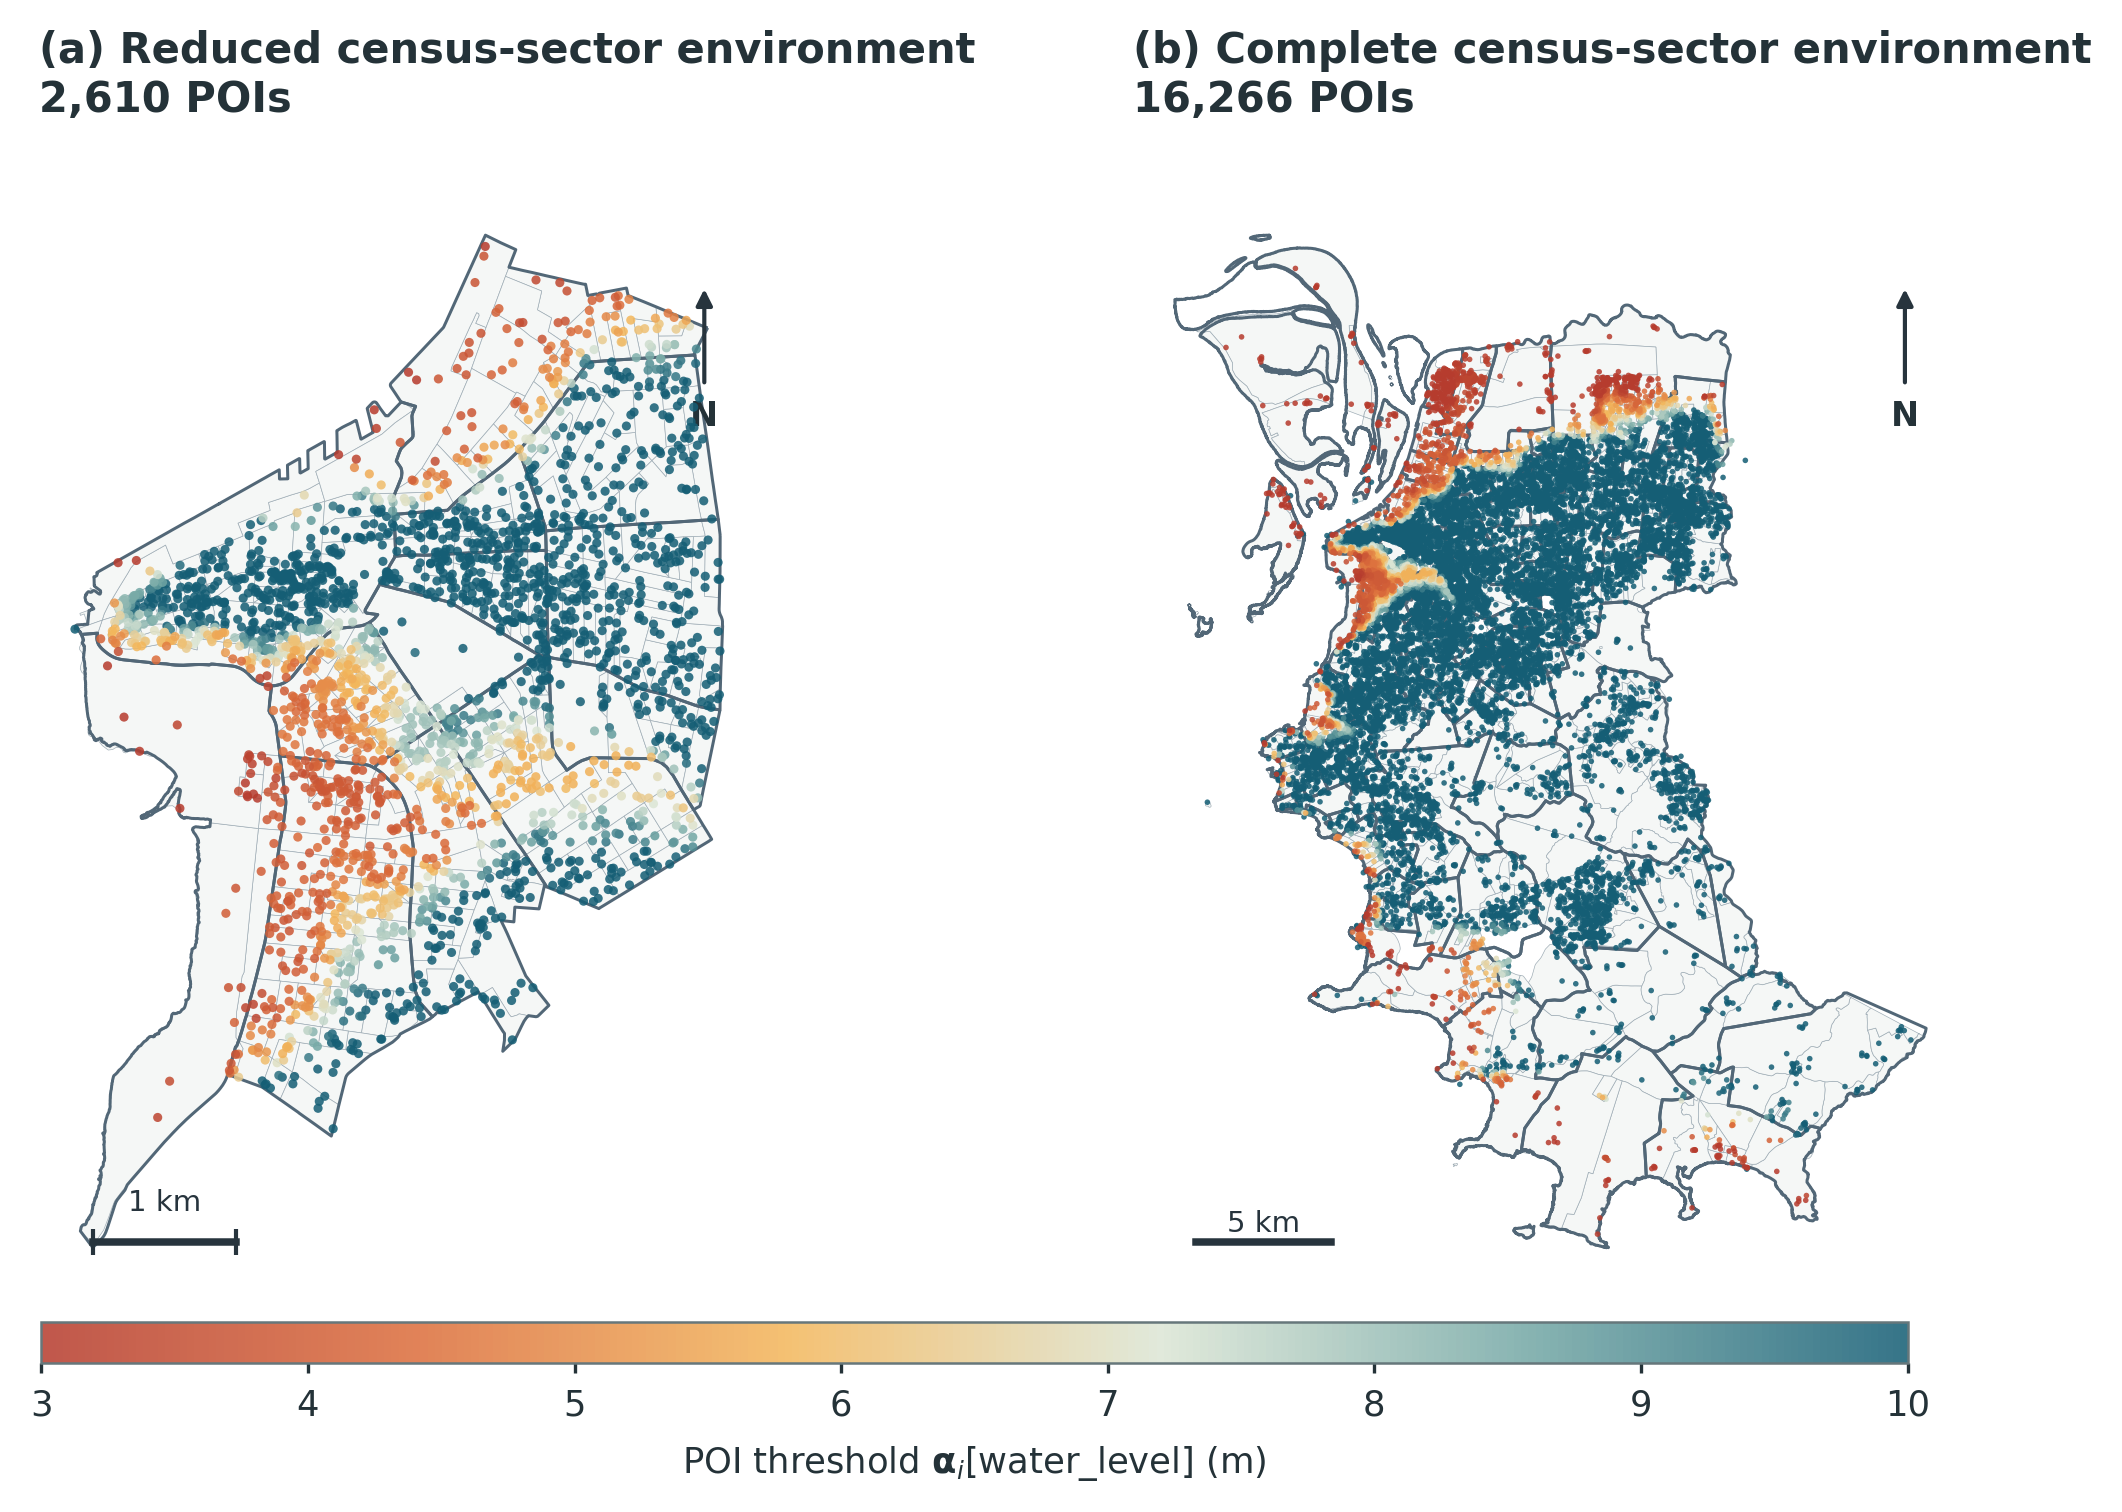
\includegraphics[width=0.99\textwidth]{fig/viz/flood_exposure_thresholds_comparison.png} 
    \caption{Spatial distribution of $P$ flood-exposure thresholds in the (a) reduced and (b) complete census-sector environments. Marker color represents $\bm{\alpha}_i[\mathrm{water\_level}]$, the minimum modeled water level at which the corresponding $P$ is treated as flooded.} 
    \label{fig:flood_exposure_thresholds} 
\end{figure}

The current water-level condition is supplied separately through the plugin configuration and may be represented by a static value or a time-varying sequence. The flood-aware mobility experiments use historical observations obtained from a public water-level dashboard\footnote{Historical water-level dashboard: \url{https://bit.ly/4wIpZPC}.}. These observations were processed into an hourly sequence compatible with the simulation time steps. Other configurations may instead use synthetic water-level values when controlled disruption conditions are required.

At each simulation step, the plugin compares the current water level with the exposure threshold of each configured $P$. When the current value reaches or exceeds the threshold, a direct disabling condition \textit{flood} is added to $C_i(t)$. When the level falls below the threshold, only this condition is removed. A $P$ therefore remains unavailable if another direct condition or an unsatisfied dependency continues to prevent its operation.

The Water-Level Data Plugin changes the state of the environment but does not itself determine how the population responds to that state. Movement suppression, destination substitution, evacuation, or other responses remain responsibilities of the plugins that execute actions involving the affected locations.


%GA: posso combinar com o texto inicial, mas pensei em deixar aqui após comentar a ideia de availability e de desabilitar Ps. E destacar que tem opções distintas de configurações
\subsubsection{Popular Times and L\'evy Walk Plugins: Mobility Policies under $P$ Unavailability} 
\label{sec:availability_aware_mobility_plugins} 

The Popular Times and L\'evy Walk plugins described in Section~\ref{sec:normal_life} can account for $P$ availability when processing normal-life movement. This allows environmental disruptions to affect recurring mobility.

The \textit{Popular Times Plugin} can suppress an activity request when its origin or requested destination is unavailable. It also provides an optional destination-substitution policy in which an unavailable destination is replaced by an available $P$ of the same type. In this case, the plugin retains both the requested and receiving destinations, allowing redirected demand to remain distinguishable from demand originally associated with the alternative location. 

The \textit{L\'evy Walk Plugin} can likewise account for unavailable origins and destinations. In the attendance-based configuration used for work and school mobility, requests that cannot be completed because of $P$ availability are retained as unmet demand.
The plugin records the information required to distinguish requested, fulfilled, and interrupted mobility and to preserve the original home associated with the population.

These responses are configuration and policy choices rather than intrinsic semantic restrictions of the mobility plugins. For example, the experiments in this thesis allow substitution for selected activity destinations while treating unavailable work and school destinations as unmet commute demand. Other simulations may configure different destination types or response policies according to their modeling objectives. %This separation between environmental state and mobility response allows the same flood condition to be combined with different assumptions about how populations adapt to unavailable locations.


\subsubsection{Shelter Plugin} \label{sec:shelter_plugin_inputs} 

The \textit{Shelter Plugin} represents evacuation and temporary accommodation of populations affected by an environmental disruption. In contrast to mobility suppression or destination substitution, sheltering introduces new movement in response to population exposure. The plugin combines information about exposed populations with the locations, capacities, occupancies, and availability of shelter $P$s. 

Shelter information was collected from the Abrigos RS website on May 15, 2024\footnote{Abrigos RS: \url{https://abrigosrs.org/}.}. The collected dataset contained 128 records with names, addresses, coordinates, neighborhoods, capacities, occupancies, and free-text observations. After filtering incomplete records, the Shelter Plugin adds 104 $P$s of type \textit{shelter} to the selected base environment, with a combined recorded capacity of 12,519 people and an initial occupancy of 10,963. These shelter $P$s are therefore not part of the shared spatial representations described in Section~\ref{sec:spatial_representations}; they are introduced only when the Shelter Plugin is included in a simulation.

Figure~\ref{fig:shelter_locations_status} presents the spatial distribution and reported initial occupancy of the shelters added to the environment. In addition to illustrating the domain-specific $P$s introduced by the Shelter Plugin, the map shows the uneven spatial distribution of shelter capacity across Porto Alegre.

\begin{figure}[ht]
\centering
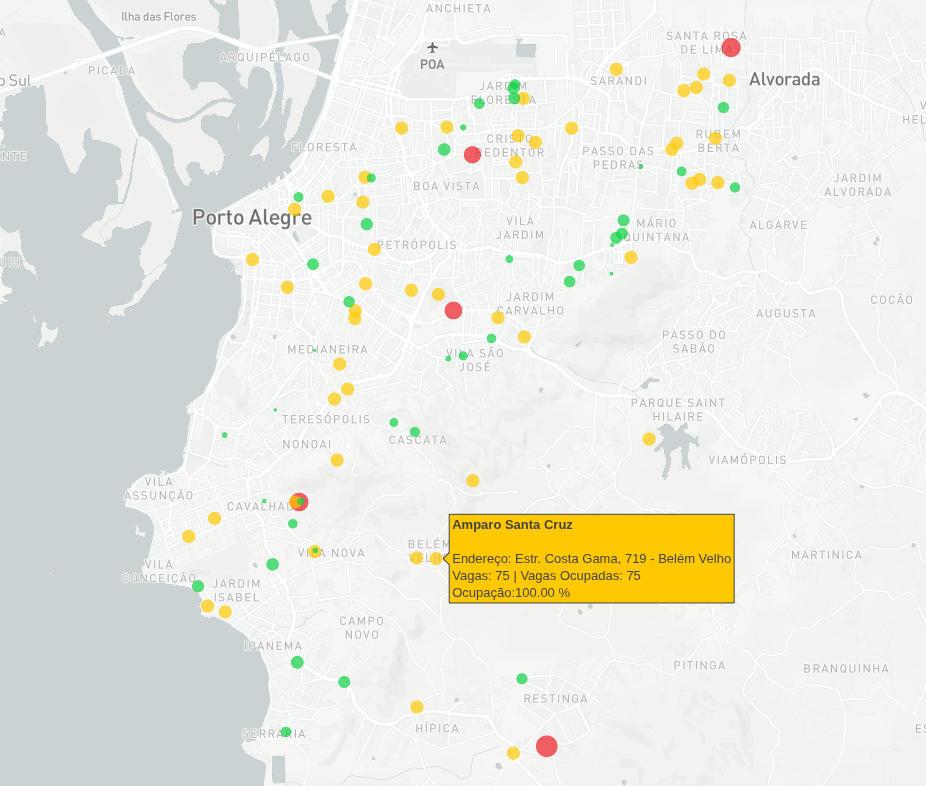
\includegraphics[width=0.85\textwidth]{fig/viz/shelters.png}
\caption{Shelter locations and reported initial occupancy in Porto Alegre. Marker color distinguishes shelters with available capacity, shelters at capacity, and shelters whose recorded occupancy exceeds their reported capacity; marker size is proportional to capacity.}
\label{fig:shelter_locations_status}
\end{figure}

Shelter coordinates, capacities, occupancies, and other facility-specific information are represented through attributes in $\bm{\alpha}_i$. Population exposure is defined separately and can therefore be configured independently from the shelter network and its available capacity. 

The plugin introduces the traceable characteristic \texttt{flooding\_status}, used to distinguish populations classified as \texttt{safe}, \texttt{in\_danger}, or \texttt{sheltered}. Because this state remains associated with population blobs, exposed, waiting, and admitted populations can coexist at the same $P$ without losing their respective conditions. 

The \textit{Shelter Plugin} comprises three principal behaviors. 
First, eligible populations in danger may be requested to move toward available shelter according to a configured evacuation policy. 
Second, populations arriving at a shelter are admitted according to its remaining capacity; those that cannot be accommodated remain in the \texttt{in\_danger} state. 
Third, an optional reallocation mechanism can transfer waiting populations from a full or unavailable shelter to other available facilities with remaining capacity. 

Shelter capacity and $P$ availability are represented separately. A shelter reaching its capacity is not automatically considered unavailable; instead, additional admission is rejected by the shelter policy. Conversely, a shelter may become unavailable because of an independent condition, such as a configured facility failure, represented through its cause set $C_i(t)$. This distinction allows service capacity, environmental conditions, and facility failures to be combined without treating them as equivalent properties of the environment.

%The plugin can be configured with parameters controlling population exposure, evacuation response, capacity, reallocation, and facility availability. 
%The particular exposure conditions, response rates, capacity variations, failure configurations, execution schedule, and other experimental choices are defined later in the corresponding simulation setup.


\subsection{Health-Related Processes and Services}
\label{sec:health_processes_services}

The preceding extensions primarily introduce or modify population movement. Health-related scenarios additionally require changes in population state and access to recurring services. In this work, these requirements are represented through plugins for epidemic contagion, vaccination, and dialysis treatment, together with mechanisms for representing dependencies between healthcare facilities and supporting urban infrastructure.

The epidemic plugins operate directly on the population represented at each $P$, allowing health states to evolve as different population groups share locations over time. The dialysis plugin instead introduces recurring treatment demand and selects among available service locations according to their schedules, capacities, and infrastructure dependencies. 
Although these applications address different processes, both illustrate how domain-specific state and behavior can be added without modifying the general definitions of population blobs, $P$s, or regions. The specific epidemiological parameters, vaccination configurations, treatment demand, service capacities, and disruption scenarios adopted in the experiments are presented later in their respective simulation setups.

\subsubsection{Infection Plugin}
\label{sec:infection_plugin_inputs}

The \textit{Infection Plugin} represents epidemic contagion using a susceptible--infected--removed (SIR) model~\cite{kermack1927contribution}. Through its model extension, the plugin introduces a traceable characteristic representing the SIR state, with the possible values \texttt{susceptible}, \texttt{infected}, and \texttt{removed}. The removed state indicates that a population no longer participates in contagion and does not distinguish recovery, immunity, and mortality as separate outcomes.

Because the SIR state is traceable, populations with different epidemiological states remain distinct when they occupy the same $P$. At each contagion update, the plugin evaluates the susceptible and infected populations currently co-located at a $P$. For a total population $N$, the implemented dynamics follow

\begin{equation}
   \frac{dS}{dt}=-\frac{\beta I S}{N},
\end{equation}

\begin{equation}
   \frac{dI}{dt}=\frac{\beta I S}{N}-\gamma I,
\end{equation}

\begin{equation}
   \frac{dR}{dt}=\gamma I,
\end{equation}

where $S$, $I$, and $R$ denote the susceptible, infected, and removed populations, respectively, while $\beta$ and $\gamma$ represent the infection and removal rates. The corresponding basic reproduction number is given by $R_0=\beta/\gamma$.

The plugin configuration specifies the epidemiological parameters and the initial infected population. Since contagion is evaluated during simulation execution, population movement changes which groups share a $P$ and consequently which populations participate in each local infection update. Fractional transitions resulting from the aggregate SIR calculations are retained between evaluations and subsequently converted into integer population quantities while preserving the represented population.

The Infection Plugin can also access information supplied by other plugins. In the vaccination experiments, vaccine effectiveness modifies the susceptible-to-infected transition according to the vaccination state of the population. %The particular initialization, epidemiological parameters, execution frequency, and mobility conditions used in each experiment are specified in the corresponding simulation setup.

\subsubsection{Vaccination Plugin}
\label{sec:vaccination_plugin_inputs}

The \textit{Vaccination Plugin} represents the allocation of vaccine doses and the progressive vaccination state of the population. It introduces the traceable characteristic \texttt{vaccine\_level}, whose value records the vaccination level attained by each population blob. Because this characteristic is preserved during movement and blob operations, populations with different vaccination states can remain distinguishable throughout the simulation.

The plugin configuration defines the number of vaccination levels (i.e. doses), the effectiveness associated with each level, the conditions under which subsequent doses become available, and the temporal series of available doses to be applied. When a vaccination request is processed, eligible population is selected, its vaccination level is updated, and the resulting state remains associated with that population after it returns to its previous location.

The vaccination quantities used in this thesis are based on the daily Porto Alegre series obtained from the Rio Grande do Sul vaccination dashboard\footnote{Rio Grande do Sul COVID-19 vaccination dashboard: \url{https://vacina.saude.rs.gov.br/}.}. The source reports doses applied by date and provides an observed temporal input. In the simulations, the distribution of these quantities among the modeled population is controlled by the vaccination plugin and its scenario configuration.

Additionally, vaccination state can be accessed by extensions. In the epidemic experiments, the Infection Plugin uses the effectiveness associated with the current vaccination level to modify modeled susceptibility. %The effectiveness values, dose schedules, allocation policy, and other experimental choices are defined in the corresponding simulation setup.

\subsubsection{Dialysis Plugin}
\label{sec:dialysis_plugin_inputs}

The \textit{Dialysis Plugin} represents access to recurring, capacity-constrained treatment. Unlike occasional service demand, dialysis requires patients to return periodically for treatment, so temporary limitations in clinic availability or capacity may produce demand that remains unresolved after the original treatment time. 

The infrastructure required by the dialysis experiments is not part of the base census-sector environments. When the dialysis-related extensions are loaded, domain-specific $P$s representing dialysis clinics and supporting water-treatment facilities are added to the selected spatial representation.

The plugin configuration defines the population requiring treatment, the interval between treatments, the $P$ types representing patient origins and dialysis clinics, and the service schedules and treatment capacities associated with the clinics. Default schedule and capacity values can be provided for the clinic type, while clinic-specific configurations allow individual facilities to use different operating intervals or capacities without changing the treatment mechanism. 
%The clinic schedules and treatment capacities used in the experiments are scenario-defined parameters rather than observed estimates of service operation.

The plugin extends the population representation with traceable characteristics required to preserve the treatment lifecycle. These include whether a population requires dialysis, its treatment frequency, next due date, current treatment status, residence origin, and treatment progression. Initial due dates may be distributed across the treatment interval so that recurring demand does not necessarily occur simultaneously for the entire patient population.

During simulation execution, the plugin identifies patients whose treatment is due and searches for an eligible clinic. Clinic eligibility combines several conditions: the facility must be available according to $C_i(t)$ and $D_i$, it must be operating at the current simulation step, and it must have remaining treatment capacity. Among eligible facilities, the extension selects a geographically suitable clinic and moves the corresponding population for treatment. After treatment is completed, patients return to their origin, while patients who cannot be admitted remain due and may be reconsidered during subsequent simulation steps.

These conditions distinguish service operation from $P$ availability. A clinic outside its opening interval or with exhausted treatment capacity remains an available $P$ but cannot accept additional treatment at that time. A clinic affected by a direct unavailability condition or an unsatisfied infrastructure dependency, in contrast, is unavailable to the treatment action.

\subsubsection{Dependency-Mapping Plugin}
\label{sec:dependency_mapping_plugin_inputs}

Dialysis services are also used to exercise the dependency component $D_i$ of each $P_i$. The \textit{Dependency-Mapping Plugin} constructs relationships between service $P$s and the infrastructure required for their operation. In our experiments, dialysis clinics depend on water-treatment facilities, represented as $P$s of type \textit{water source}.

The resulting infrastructure overlay contains dialysis clinics and water-treatment stations (\textit{Estações de Tratamento de Água}, ETAs), represented as additional $P$s of type \textit{dialysis clinic} and \textit{water source}, respectively. ETA locations and the association of neighborhoods with water-supply systems were derived from information published by the Municipal Department of Water and Sewage (DMAE)\footnote{DMAE water-system information: \url{https://prefeitura.poa.br/dmae/informacoes-agua}.}. The complete overlay contains six water-treatment stations and 12 dialysis clinics.

Figure~\ref{fig:dialysis_network} illustrates the dialysis infrastructure represented in the environment and the relationships between clinics and their supporting water sources. The clinic-centered view identifies the water sources on which a selected clinic depends, while the water-source-centered view highlights the neighborhoods supplied by a selected source. 

\begin{figure}[!ht]
    \centering

    \begin{subfigure}{\linewidth}
        \centering
        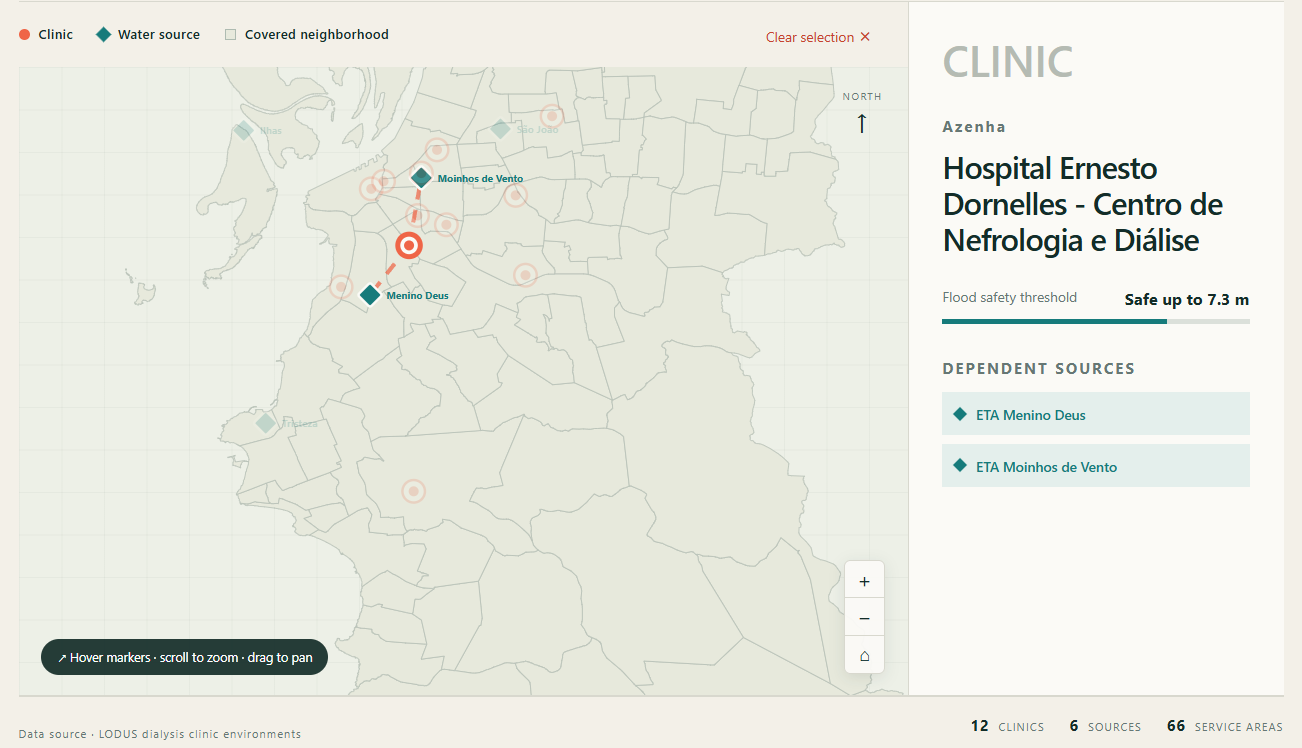
\includegraphics[width=\linewidth]{fig/viz/dialysis_viz_clinic.png}
        \caption{Clinic-centered view showing the water sources supporting a selected dialysis clinic.}
        \label{fig:dialysis_network_clinic}
    \end{subfigure}

    \vspace{0.5em}

    \begin{subfigure}{\linewidth}
        \centering
        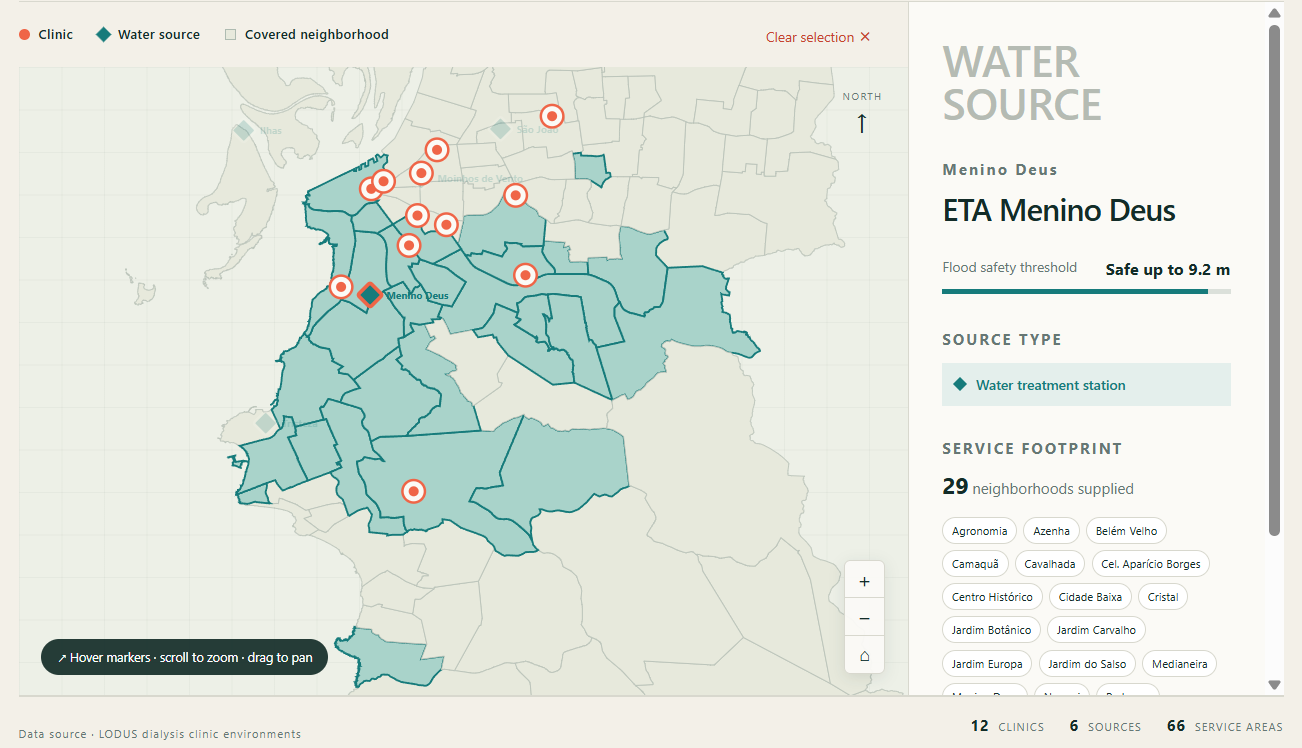
\includegraphics[width=\linewidth]{fig/viz/dialysis_viz_eta.png}
        \caption{Water-source-centered view showing the neighborhoods supplied by a selected water source.}
        \label{fig:dialysis_network_source}
    \end{subfigure}

    \caption{Visualization of the dialysis infrastructure represented in the Porto Alegre environment. 
    (a) Selecting a dialysis clinic identifies its supporting water sources, illustrating the relationships represented by its dependency rules \(D_i\). 
    (b) Selecting a water source highlights its service footprint across the environment.}
    \label{fig:dialysis_network}
\end{figure}

Dialysis clinic locations and their relations to water sources were defined as inputs to the health-service representation. Names, coordinates, external identifiers, and the identifiers used to associate clinics with water sources are stored in the attribute mapping $\bm{\alpha}_i$ of each corresponding $P_i$.

The plugin interprets these attributes when the environment is initialized and constructs the associated dependency rules in $D_i$. The dependency configuration determines which $P$ types act as dependent facilities and supporting resources, how they are matched, and how many supporting $P$s must remain available for the dependency to be satisfied. The generic environment mechanism subsequently evaluates these rules, so the plugin is responsible for constructing the relationships rather than implementing a dialysis-specific availability mechanism.

As a result, a direct disruption to a water-source $P$ may indirectly make one or more dialysis clinics unavailable without adding the same direct cause to those clinics. This separation allows the dependency structure to be reused with different disruption mechanisms.

\subsubsection{Scheduled-Availability Plugin}
\label{sec:scheduled_availability_plugin_inputs}

The \textit{Scheduled-Availability Plugin} provides a generic mechanism for changing $P$ availability at configured simulation steps. It schedules actions that add or remove a named direct disabling condition from the cause set $C_i(t)$ of the corresponding $P_i$, allowing temporary or persistent facility outages to be represented independently of the service-specific plugins that use those locations.

In the dialysis scenarios, this mechanism is used to represent controlled outages of water sources or clinics through the direct condition \texttt{off\_cycle}. Because individual conditions are stored independently in $C_i(t)$, removing a scheduled-outage condition does not restore a $P$ when another condition remains active. Similarly, restoring a water source only restores dependent clinics when their dependency rules in $D_i$ become satisfied and the clinics have no remaining direct disabling condition.

The Scheduled-Availability Plugin can therefore be composed with the Water-Level Data Plugin introduced in Section~\ref{sec:water_level_plugin_inputs}. Flooding and scheduled outages remain distinct direct conditions, while infrastructure dependencies propagate the resulting availability state to dependent facilities. %The particular outage locations, execution times, recovery conditions, and combinations with flooding used in the dialysis experiments are specified in their simulation setup.




\section{Input Provenance and Interpretation}
\label{sec:input_provenance_summary}

Because the experiments combine externally sourced data, derived spatial attributes, and scenario-defined parameters, their provenance must be considered when interpreting the results. This distinction is particularly important when experimental inputs are used to test model behavior rather than to reproduce observed conditions in Porto Alegre.
Table~\ref{tbl:simulation_data_provenance} summarizes the role and sources of the principal data families in the same general order in which they are introduced above.

\begin{table}[ht]
\centering
\footnotesize
\setlength{\tabcolsep}{4pt}
\caption{Provenance and interpretive status of the principal environment and scenario-input families.}
\label{tbl:simulation_data_provenance}
\begin{tabularx}{\linewidth}{@{}p{3.5cm}p{6.2cm}X@{}}
\toprule
\textbf{Data family} & \textbf{Documented basis} & \textbf{Interpretive status} \\
\midrule

Neighborhood geometry and $P$s
& City Hall boundaries and OpenStreetMap amenities
& Externally sourced spatial data used to construct the neighborhood-level environment. \\

Neighborhood population
& IBGE, ObservaPOA, and PROCEMPA
& Externally sourced demographic data used to initialize the population represented in each neighborhood. \\

Census-sector environments
& IBGE 2022 geometries and aggregates
& Official census data spatially processed to construct the finer-grained population and $P$ representation. \\

L\'evy Walk parameters
& Scenario-defined behavioral and routine parameters
& They support controlled mobility comparisons and are not calibrated estimates of observed Porto Alegre trajectories. \\

Popular Times profiles
& Type-specific temporal profiles derived from patterns observed in Google Maps Popular Times
& Derived temporal-demand profiles rather than measured visitation counts for individual establishments. \\

Large-scale event inputs
& Existing modeled event locations with scenario-defined event times and attendee requests
& The request of 500,000 attendees per event is a stress parameter rather than an observed attendance value. \\

Contagion parameters
& Reported $R_0$ values from studies of COVID-19 transmission in Brazil; remaining epidemic and restriction parameters configured by scenario
& The experiments provide controlled comparisons rather than calibrated epidemiological forecasts. \\

Vaccination quantities
& Applied-dose series from the Rio Grande do Sul vaccination dashboard
& Observed daily vaccination quantities; doses are distributed among modeled regions in proportion to their populations.\\

Flood thresholds and exposure
& Climate Central simulated water-level map evaluated at the coordinates of modeled $P$s
& Derived exposure attributes representing the minimum modeled water level at which each location becomes inundated.\\

Water-level
& Public Power BI records from May--June 2024 plus synthetic stress sequences
& Historical observations are used for flood-mobility scenarios, while synthetic sequences are used for controlled stress experiments.\\

Shelters
& Abrigos RS snapshot collected on May 15, 2024
& Historical snapshot of shelter locations, capacities, and occupancies; the original source is no longer available online. \\

ETAs and dialysis clinics
& DMAE water-system information; clinic data and dependency definitions
& Infrastructure locations and dependencies provide the scenario topology, while clinic schedules and hourly treatment capacities are synthetic experimental parameters. \\
\bottomrule
\end{tabularx}
\end{table}

%SO: re-escrevi e tirei o uncertanty porque acho que merece uma discussao nas finals
%Across the following results, externally sourced coordinates, population quantities, and capacities provide geographic and operational context, while behavioral parameters, demand volumes, failures, environmental conditions, and policy responses define the comparisons being tested. Consequently, uncertainty in the source data and uncertainty due to stochastic simulation represent different aspects of the experiments.
Across the experiments presented in the following chapter, externally sourced data provide the spatial, demographic, and service context of Porto Alegre, while scenario-specific parameters define the mobility patterns, disruptions, demands, and responses to be evaluated. This distinction allows the same underlying environments to support different experimental conditions and provides a common basis for interpreting the simulation results.




    

\begin{comment}
    

%SO: re-escrevi abaixo, podes ver comentários na parte comentada. Estava muito com cara de manual; Revisar para validar
\section{OLD:Routine Mobility Inputs}
\label{sec:behavioral_policy_input_data}

Routine mobility provides the baseline movement patterns of the simulated population. These movements represent the daily activities performed by individuals under normal conditions and serve as the basis upon which other processes, such as large-scale events, epidemics, or environmental disruptions, may introduce additional mobility demands. Two complementary mobility models are considered in the core model of this thesis: a stochastic L\'evy Walk model
and a model based on temporal activity profiles derived from Popular Times.

\paragraph{L\'evy Walk:}

The L\'evy Walk model %SO: ref
represents routine mobility through configurable
behavioral parameters rather than observed trajectories. Its objective is to
produce realistic baseline movement patterns while allowing controlled
experiments under different mobility conditions. The input parameters include
the heavy-tailed travel-distance scale, packet size, mobility restriction
factor, worker attendance rate, student attendance rate, departure-hour
profiles, and visit durations.

These parameters configure the mobility model adopted in the core model,
while the corresponding plugin introduces the additional mobility-related
state and behaviors required to represent commuting activities.

\paragraph{Popular Times:}

This thesis proposes a routine mobility model driven by temporal activity
profiles inspired by the Popular Times feature of Google Maps. The model
captures how the demand for different categories of urban activities varies
throughout the week and uses this information to generate routine mobility
patterns. Three weekly hourly profiles are considered, corresponding to
marketplaces, restaurants, and pharmacies. These profiles were constructed
from the temporal activity patterns observed in the Popular Times feature of
Google Maps.

Unlike the stochastic destination selection adopted by the L\'evy Walk model,
the proposed Popular Times model directly represents the temporal demand for
different categories of points of interest. Consequently, the likelihood of
visiting each type of location varies according to the day of the week and
hour of the day, producing routine mobility patterns that better reflect the
temporal dynamics of urban activities.

\paragraph{Large-scale events.}

Large-scale events introduce temporary concentrations of population at
specific locations and times. Each event is characterized by its scheduled
time, destination point of interest, and expected number of participants.
Event locations correspond to existing points of interest in the modeled
environment, while attendance values are defined according to the scenario
being evaluated rather than historical observations.

These inputs define the event scenarios considered in this thesis and are
later interpreted by the event plugin to generate the corresponding
population movements.



%SO: parei aqui

\paragraph{Contagion and vaccination.}
The contagion experiments combine mobility with infection, vaccination, and restriction parameters in the same population representation. Epidemic initialization, homogeneous infection and removal parameters, vaccine-effectiveness values, dose-start days, and restriction levels define comparative scenarios. The three reported $R_0$ values are based on studies of COVID-19 transmission in Brazil~\cite{dutra2020covidR0,deSouza2020covirR0,dutra2021covidR0}, while the daily vaccination quantities follow the 546-value Porto Alegre series obtained from the Rio Grande do Sul vaccination dashboard\footnote{Rio Grande do Sul COVID-19 vaccination dashboard: \url{https://vacina.saude.rs.gov.br/}.}. The dashboard reports doses applied by date, and the simulation distributes the daily Porto Alegre quantities among modeled regions in proportion to their populations.

The epidemiological, restriction, effectiveness, and dose-distribution values form $\bm{\theta}_{\Pi}$. Infection and vaccination states are traceable characteristics declared through $E_{\Pi}$, ensuring that actions can select them through $\bm{T_{Tc}}$ and that blobs with different states remain distinct during merging. Registered handlers and time-step hooks in $\mathcal{F}_{\Pi}$ and $\mathcal{H}_{\Pi}$ implement infection transitions and vaccination updates.

\subsection{Environmental-Disruption Events}

%SO: re-escrevi, valide!
Environmental disruption events illustrate how a hazard can alter the availability of locations, suppress or redirect routine mobility, and create demand for capacity-constrained shelters. The proposed mechanism can accommodate different types of hazards, such as floods or fires, provided that the corresponding spatial exposure and hazard conditions are defined. In the present work, we focus on flood scenarios, motivated by the increasing impact of extreme weather events in Rio Grande do Sul, Brazil.

%The environmental-disruption events represent how a hazard situation can change the availability of locations, suppress or redirect routine mobility, and create demand for capacity-constrained shelters. While all haazard event can be simulated, in the present wotk we focused on Flood scenarios due to the impact of climate changes in our regio (RS, Brazil). %exposure is therefore represented separately from the water-level condition applied over time, allowing the same spatial environment to be evaluated under different disruption scenarios.

\subsubsection{Flood Exposure and Water-Level Scenarios}
\label{sec:flood_water_input_data}

The flood experiments instantiate this general environmental-disruption mechanism by combining two complementary inputs: the susceptibility of each modeled location to flooding and the water-level conditions associated with a simulation scenario.

Flood susceptibility is represented by assigning each $P$ a location-specific exposure threshold. This threshold is stored in the $P$ attribute $\bm{\alpha}_i[\mathrm{water\_level}]$ and indicates the minimum water level at which the location is considered flooded. Despite the key name, this value is a location-specific exposure threshold rather than the water level currently applied to the simulation. 

%The flood experiments combine a spatial representation of $P$ exposure with temporal or static water-level conditions. This separation allows flood intensity to vary between scenarios without modifying the underlying locations or their exposure thresholds.
%Flood exposure is represented through the $P$ attribute $\bm{\alpha}_i[\mathrm{water\_level}]$. Despite the key name, this value is a location-specific exposure threshold rather than the water level currently applied to the simulation. 
The spatial thresholds, in the present simulations, were collected using the simulated ``Water Level'' map provided by Climate Central's Coastal Risk Screening Tool\footnote{Climate Central Coastal Risk Screening Tool, configured for water level above mean higher high water, contiguous inundation, and the best available elevation model: \url{https://coastal.climatecentral.org/map/12/-51.1996/-30.0653/?theme=water_level&map_type=water_level_above_mhhw&basemap=roadmap&contiguous=true&elevation_model=best_available&refresh=true&water_level=5.3&water_unit=m}.}. The latitude and longitude of each $P$ were inspected on the map at successive water levels. The threshold assigned to a $P$ is the minimum water level at which its location was shown as inundated. The resulting environment files contain thresholds from 3.0~m to 10.0~m.

%The temporal or static forcing belongs to the water-level plugin configuration $\bm{\theta}_{\Pi}$. 
%SO: frase acima estranha forcing é muito feio- mudei - valide
The water-level condition is specified separately as part of the flood-plugin configuration $\theta_\Pi$.
Depending on the experiment, it can be represented by a time-varying sequence or a static value. At each simulation step, the plugin compares the current water level with the exposure threshold stored for each $P$. When the current level reaches or exceeds the threshold, the plugin adds the named cause flood to $C_i(t)$; when the water level falls below the threshold, only that cause is removed. A $P$ therefore remains unavailable if another direct cause or an unsatisfied dependency is still present.

This separation between spatial exposure and the hazard condition allows the same environment to be evaluated under different flood scenarios without modifying its underlying spatial representation. More generally, it illustrates how the environmental-disruption mechanism separates the spatial characteristics of locations from the conditions imposed by a particular hazard scenario. The resulting availability state does not itself prescribe a population response: suppression, waiting, or redirection remains determined by the action handler associated with the corresponding experiment.

%At each simulation step, the plugin compares the current forcing with $\bm{\alpha}_i[\mathrm{water\_level}]$. When the forcing reaches or exceeds the threshold, the plugin adds the named cause \textit{flood} to $C_i(t)$; when the condition no longer holds, it removes only that cause. A $P$ consequently remains unavailable while any other direct cause or unsatisfied dependency is present. This procedure converts the spatial flood map into a reusable $P$ vulnerability attribute without defining a universal mobility response: suppression, waiting, or redirection remains the policy of the action handler consuming the affected request.

The census-sector environments %SO: o que é census=sector environments que store dados? me perdi na arquitetura....
store a threshold for every modeled $P$, allowing the same flood-cause mechanism to be applied selectively to any configured $P$ type $\tau_i$. The flood-aware mobility experiments use historical observations collected from a public Power BI dashboard\footnote{Historical water-level dashboard: \url{https://bit.ly/4wIpZPC}.}. The processed hourly sequence supplies the time-varying values in $\bm{\theta}_{\Pi}$ and reproduces the rise and recession of the flood. The shelter experiments instead use a static exposure overlay in which census sectors intersecting the modeled 5.30~m flood extent define 438 exposed sectors containing 186,522 residents.

Figure~\ref{fig:flood_state_visualization} illustrates the historical flooding %SO: onde??????
and the corresponding spatial availability of $P$s at the maximum water level represented in the sequence.

%SO: arrumar o caption para colocar direita, esquerda da fig
\begin{figure}[ht]
\centering
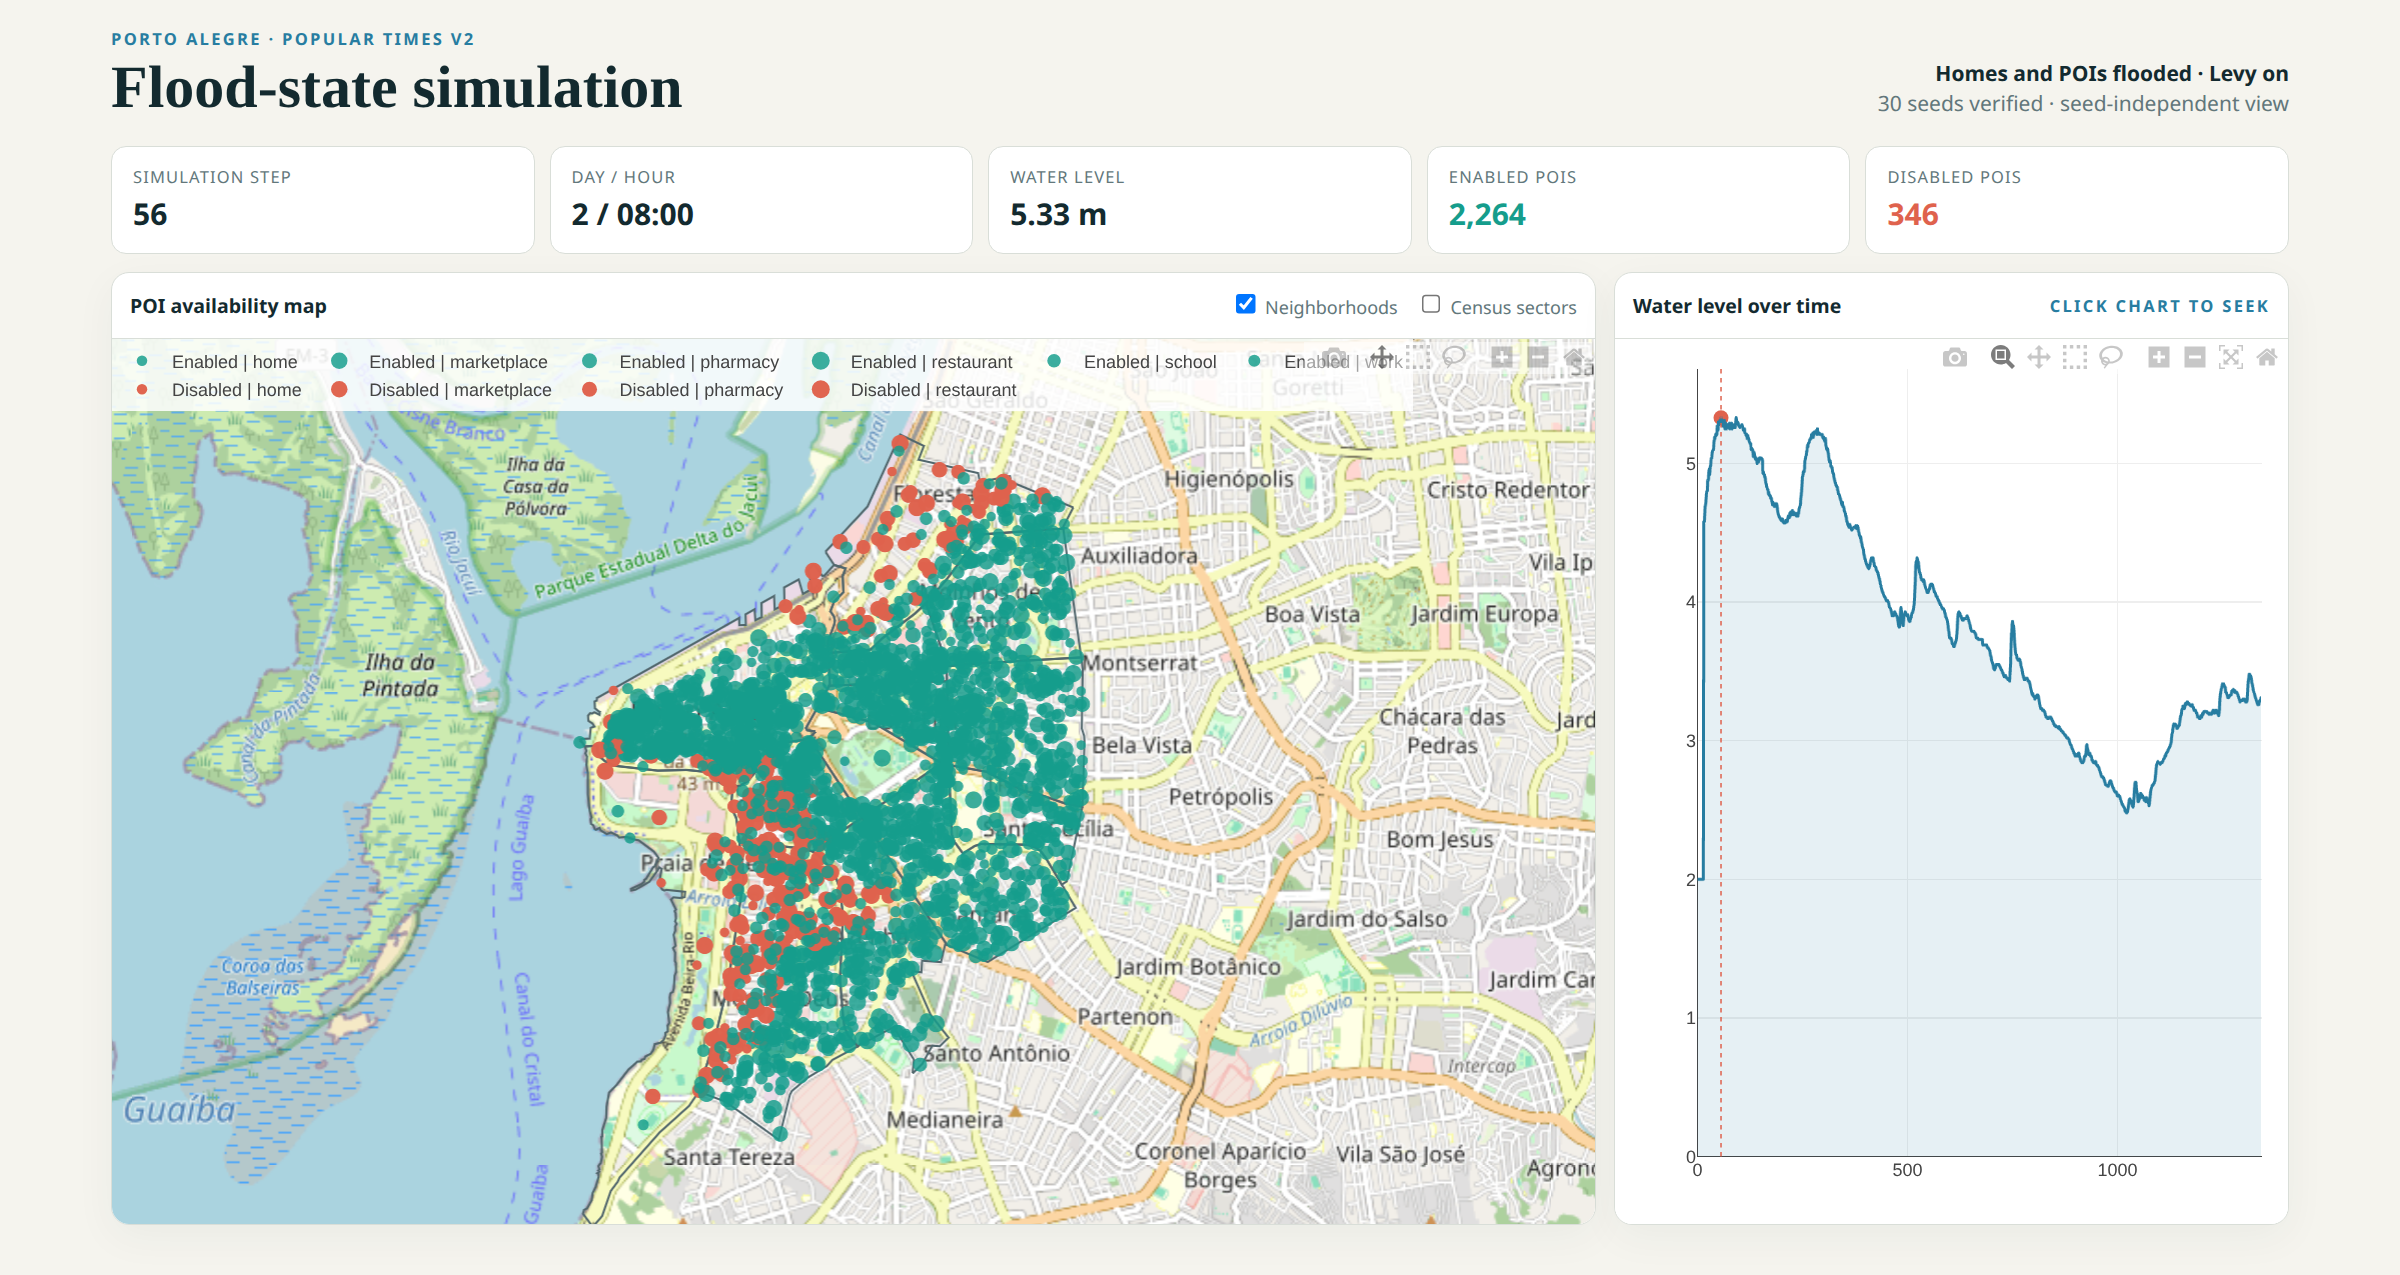
\includegraphics[width=0.99\textwidth]{fig/viz/flood_state_13_levy_both.png}
\caption{Flood-state snapshot for the reduced census-sector environment with L\'evy Walk enabled and the flood cause applied to home and activity $P$s. At simulation step 56 (day 2, 08:00), the historical sequence
%SO: sequence of what??????????????????????????????
reaches 5.33~m and makes 346 of the 2,610 modeled $P$s unavailable. The map distinguishes available $P$s from those carrying the flood disable cause.}
\label{fig:flood_state_visualization}
\end{figure}

\subsubsection{Shelter Locations and Capacities}

The shelter experiments examine whether populations displaced from flood-exposed areas can be redistributed to available emergency accommodation under spatial and capacity constraints. Their inputs, therefore, describe both the locations of shelters and the number of additional residents each shelter can accommodate.

The geographic coordinates, capacities, and occupancies of shelters were collected from the Abrigos RS website on May 15, 2024\footnote{Abrigos RS: \url{https://abrigosrs.org/}.}. The shelter locations were obtained from the geographic information available on the website. The collected input contains 128 tabular records with names, addresses, %SO: de pessoas?
coordinates, neighborhoods, capacities, occupancies, and free-text observations. After filtering and treatment of missing values, we consider 104 shelters with a combined capacity of 12,519 people and an initial occupancy of 10,963.

%SO: não gostei do proximo paragrafo. Re-escrevi. Validar
%The retained records are instantiated as $P$s of type \textit{shelter}. %SO: frase estranha retained records
%Their identifiers, %SO: their who? shelters? people?
%coordinates, reported capacities, and initial occupancies are stored through conventions for $\bm{\alpha}_i$ declared by the shelter plugin. Capacity and displacement parameters form $\bm{\theta}_{\Pi}$, while the handlers and hooks in $\mathcal{F}_{\Pi}$ and $\mathcal{H}_{\Pi}$ determine admission, denial, reallocation, and return behavior. These values therefore remain plugin-interpreted service state rather than universal fields with behavior fixed by the core environment.

The 104 shelters are represented as $P$s of type \textit{shelter}, with their geographic coordinates, capacities, and initial occupancies included as $P$ attributes ($ \ bm {\ alpha} _ i$). The shelter plugin uses these attributes together with scenario-specific capacity and displacement parameters ($\bm{\theta}{\Pi}$) to model the accommodation of displaced populations, including admission, denial due to capacity constraints, reallocation to alternative shelters, and return behavior. In this way, shelter-specific data and behavior are introduced through the plugin without modifying the general representation of $P$s in the LodusPop core model.

Figure~\ref{fig:shelter_locations_status} presents the locations and reported initial occupancy status of shelters with available capacity and occupancy information. The map makes visible both the uneven spatial distribution of shelter capacity and the limited number of places available before any simulated evacuation occurs.

\begin{figure}[ht]
\centering
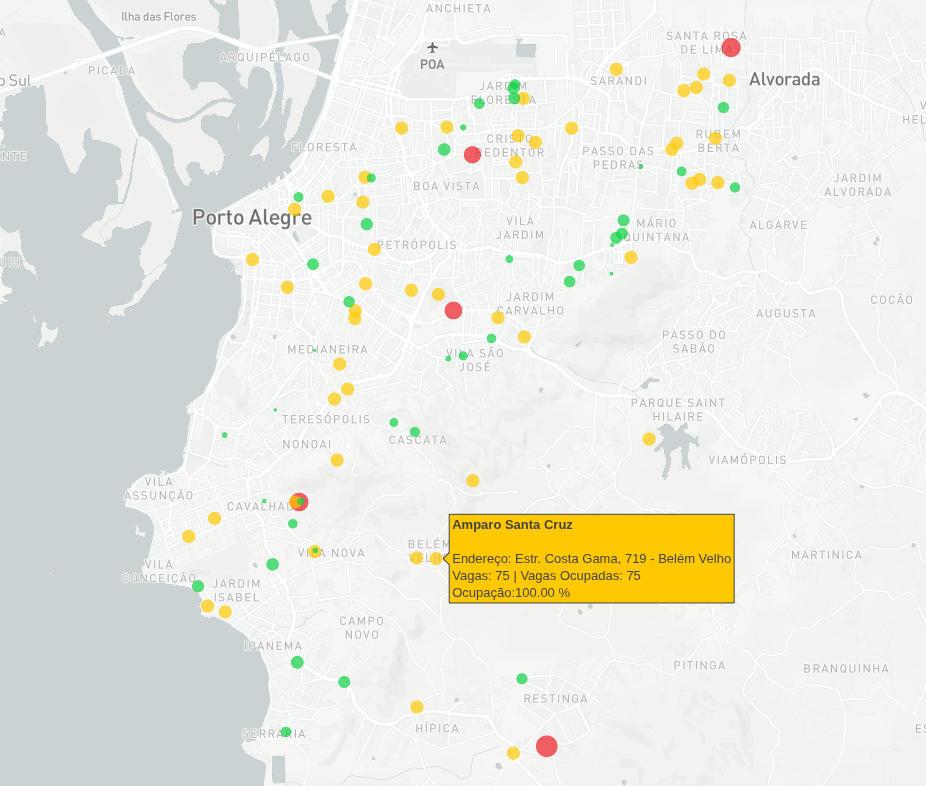
\includegraphics[width=0.85\textwidth]{fig/viz/shelters.png}
\caption{Shelter locations and reported initial occupancy status in Porto Alegre. Green markers identify shelters with available places, yellow markers identify shelters at their recorded capacity, and red markers identify shelters whose recorded occupancy exceeds their recorded capacity. Marker size is proportional to recorded capacity. The highlighted Amparo Santa Cruz record illustrates the address, capacity, occupied places, and utilization reported for an individual shelter.}
\label{fig:shelter_locations_status}
\end{figure}

\subsection{Health-Services}
\label{sec:infrastructure_input_data}

The health-service experiments examine access to recurring, capacity-constrained dialysis treatment in response to changes in demand and service availability. In addition to direct clinic disruptions, the scenarios represent dependencies on supporting water infrastructure, allowing failures at water-treatment facilities to indirectly affect access to dialysis services.

The dialysis environments represent Porto Alegre water-treatment stations (Estações de Tratamento de Água, ETAs) as $P$s of type \textit{water source} and dialysis facilities as $P$s of type \textit{dialysis clinic}. The complete overlay contains six ETAs and 12 clinics. ETA locations and the assignment of neighborhoods to water-supply systems were derived from maps and descriptions published by the Municipal Department of Water and Sewage (DMAE) and from a May 2024 account of water distribution and interconnections between the city's systems\footnote{DMAE water-system information: \url{https://prefeitura.poa.br/dmae/informacoes-agua}. GZH description of water distribution by neighborhood and connections between systems: \url{https://bit.ly/3TOMmnY}.}. The six ETAs reported by DMAE correspond to the six treatment stations represented in the complete environment.

%SO: muito hifen...
%Dialysis-clinic locations and clinic-to-water-source relations were provided by colleagues of the author based on their domain knowledge and the water-supply maps and sources cited above. Each clinic-to-source relation is represented by a dependency constraint in $D_i$, whereas names, coordinates, and external identifiers are stored in the relevant $P$ attribute mappings. Clinic opening and closing times and hourly treatment capacities are synthetic scenario parameters included in $\bm{\theta}_{\Pi}$.
Dialysis clinic locations and their relations to water sources were defined as inputs to the health service scenarios.\footnote{These data were compiled from the water supply maps and sources cited above, with support from project collaborators with domain knowledge.} Each relation between a clinic and a water source is represented by a dependency constraint in $D_i$, whereas names, coordinates, and external identifiers are stored in the relevant $P$ attribute mappings. Clinic opening and closing times, as well as hourly treatment capacities, are synthetic scenario parameters included in $\bm{\theta}_{\Pi}$.

%SO: re-escrevi para tirar cara de software
%The dialysis plugin uses $E_{\Pi}$ to declare the traceable characteristics required to represent patient selection, treatment frequency, due dates, status, origin, and treatment time. Its registered handler and time-step hook in $\mathcal{F}_{\Pi}$ and $\mathcal{H}_{\Pi}$ generate recurring demand, apply clinic capacity and schedule constraints, and perform treatment and return transitions.
The dialysis plugin uses $E_{\Pi}$ to define the traceable characteristics required to represent patient selection, treatment frequency, due dates, status, origin, and treatment time. Dialysis-specific behavior is represented through $\mathcal{F}{\Pi}$ and $\mathcal{H}{\Pi}$, including recurring treatment demand, clinic capacity and schedule constraints, treatment, and patient return.

%SO: re-escrevi. Valide
%The dialysis stress tests combine these service inputs with independent mechanisms for changing $P$ availability. A scheduled water-source outage adds its own direct cause to the source's $C_i(t)$, while flood exposure adds the distinct \textit{flood} cause to each affected source or clinic. The constraints $D_i$ then propagate source unavailability to dependent clinics. Removing one direct cause cannot restore a $P$ while another cause or an unsatisfied dependency remains. Synthetic sudden-rise water-level sequences, including transitions to 9.3~m and 10.1~m, are used as controlled stress conditions rather than observed hydrographs.
The dialysis stress tests combine these service inputs with various conditions that affect $P$ availability. Water source outages and flood exposure are represented as independent causes of unavailability in $C_i(t)$, allowing multiple disruption conditions to coexist. The dependency constraints $D_i$ propagate the unavailability of water sources to the dialysis clinics that depend on them. Consequently, a $P$ remains unavailable as long as at least one direct cause or dependency constraint prevents its operation. Synthetic water level sequences, including sudden increases to 9.3~m and 10.1~m, are used to create controlled stress conditions rather than to reproduce observed flood dynamics.

\end{comment}